% !TEX root = main.tex

\section{Experiments} \label{sec:experiments}

The confidence one can have on the encoders of the robot depends on several factors from actuators' design to control strategies. 
In the legged locomotion case, this can also depend on the general design of the robot.
For example, during walking phases with humanoid robot HRP-2, one can notice a sliding phenomenon when the foot hits the ground. 
If this effect is not measured, its integration over several steps can lead to very poor motion estimates. 
We show that observing this slide and getting a better estimation of both the foot and the robot trajectories is possible with an IMU fixed on the sliding member, \ie, the robot's foot.

We use a low-cost IMU in our application to demonstrate the feasibility of our method. 
To that end, we selected the MPU6050 from Invensense, which combines triaxial accelerometers and gyrometers, provides 1kHz data rate, and is extensively used in the open source community.

\subsection{Method}


Keyframes are declared at the beginning and ending of each support phase of the selected foot. Factors active in the graph (see \figRef{fig:factor_graph}) are: initial position and yaw; zero velocity, bias drift, IMU pre-integration, and kinematic odometry. We only use the bias magnitude factors in the initial KF.

An improved version of our graph estimator incorporates an extra KF in the middle of the foot's flying phase. In this case, kinematic factors are added between all consecutive KFs, but zero-velocity factors only for those in the contact phase.

%The parameters we need to calibrate for a correct integration are the IMU biases, on top of which we integrate the incoming IMU data.
%The time varying property of the bias is a critical point to consider in order to avoid large deviations. 
%This calibration is made possible
%through the dependencies of the delta pre-integration (${\Dp}(\bfa_b, \bw_b), {\Dv}(\bfa_b, \bw_b), {\Dq}(\bw_b)$). 
%Fusing both odometer and IMU provides constraints on position and orientation parts of
%the state vector. 
%However, velocity is still not observable and is affected by the bias estimation. 
%In the case of legged locomotion, we fix the observability problem by adding a zero velocity constraint when the foot is stable on the ground.
%
%The initial orientation estimation is made possible by adding an absolute constraint on yaw part of the state vector, otherwise we would run into observability problems. \textbf{add figure here (graph)}

\subsection{Results}
\subsubsection{Trajectory reconstruction}

We first validate our fusion method on a simplified setup. We do without the robot: we attach the IMU to a walking persons's foot, and use motion capture (MOCAP) techniques to generate the kinematic constraints. 
The MOCAP provides more controlled conditions for the kinematic measurements; it is used to get odometry between zero-velocity phases, i.e. when the foot is on the ground.
\figRef{fig:forward_walk_IRI} shows the reconstructed foot trajectories for the cases without the flying KF, and with the flying KF. We can observe a correct estimation only when the flying KF is added. Bias autocalibration is also more stable with the flying KF.

%Then we show that using an IMU on the foot of the robot leads to a better estimation of the real position of the member compared to encoder based odometry. 
%We check the feasibility of the trajectory reconstruction using a 1Khz IMU attached to one's foot and tracked with a motion capture (MOCAP) system. The MOCAP is used to get odometry between zero-velocity phases, i.e. when the foot is on the ground,
%and will be taken as the ground truth against which we compare the trajectory reconstruction.
%
%We reproduce the movements the feet of a robot could have when it is walking. However, as shown in figures \textbf{add figure here}, the final optimal state
%is not the expected one and acceleration biases are rapidly changing. The variation that we can see is not only due to some random walk and can be explained by the excitement of biases in a different axis.
%As explained in \cite{roussillon2011rt}, in opposition to gyroscope biases, acceleration biases do not converge toward stable values during a motion exciting several axis of the sensor. 
%This effect can be explained by time inconsistency meaning that we fail
%to use the information of the entire motion to converge toward stable values as expected in the sensor model, but the problem may also be that the step motions do not use all the axis of the accelerometer as it should.

\begin{figure}[tb]
\centering
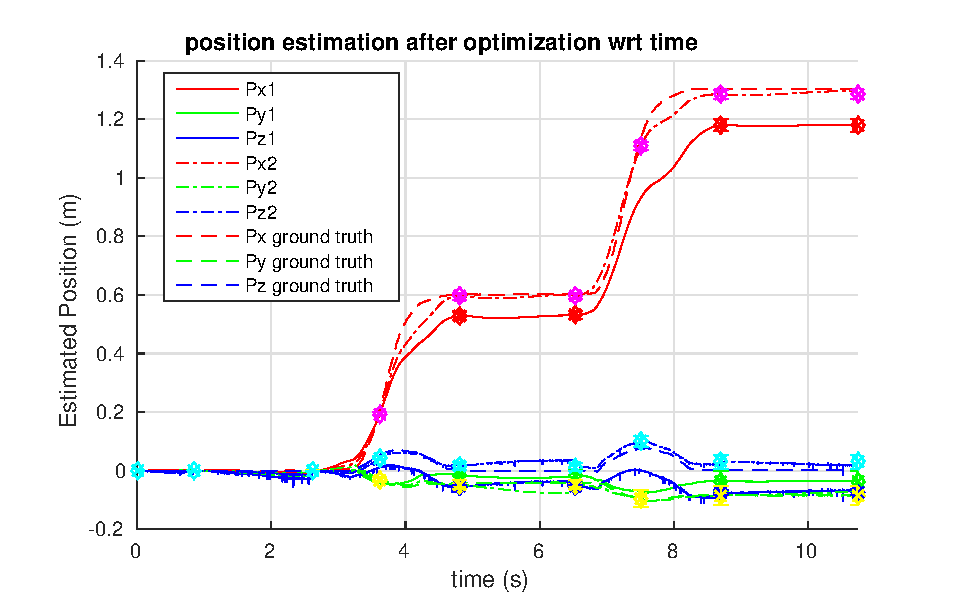
\includegraphics[scale=0.5]{figures/Result_position}
\par\vspace{4mm}
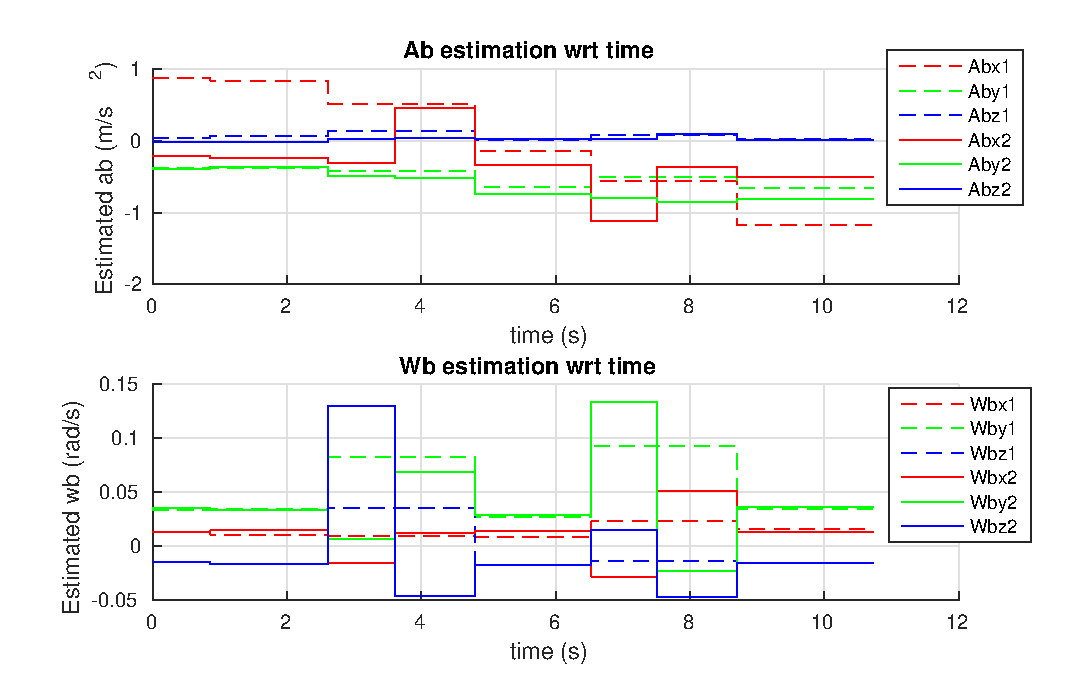
\includegraphics[scale=0.5]{figures/Result_bias}
\caption{ 
{\bf Top}: trajectory estimation during human walking with an IMU attached to a foot. Continuous, dashed and dashed-dot lines are respectively: mocap recorded ground truth, 
estimation with zero velocity constraints only, estimation using zero velocity constraint and 1 odometry measurement during foot's flying phase. odometry was here built from MOCAP information.
{\bf Bottom}: Evolution of corresponding estimated IMU biases 
}
\label{fig:forward_walk_IRI}
\end{figure}

We fix the trajectory estimation problem by adding odometry information during foot's flying phase. However, we cannot fix any other conditions making velocity and bias observation possible hence all parameters of the state vector are estimated.
This added KeyFrame reduces the integration time since last state optimization making bias random walk variation less critical on estimation. As we can see, results are much better and closer to MOCAP's ground truth as we could expect.

%TODO : process mocap experiments

\subsubsection{Legged-Locomotion's undesired behavior measurement}

We use the approach presented above in the case of the humanoid robot HRP-2 to better estimate the trajectory of the foot. This also results in a better estimation of the pose of the robot using its kinematic chain. 
For this experiment, the robot is moving in open loop and some particularities are worth to be noted compared to the previous experiment. 
The structure of the robot produces vibrations that are measured by the IMU, thus explaining the over noisy aspect of the data. The foot's flying phase is set to last 800 ms. The double support phase lasts only 20 ms, thus it is difficult to observe
even with the IMU working at 1 KHz because of the vibration it will measure on impacts.




%TODO experiment : step motion + complex rotation, followed by MOCAP


